\documentclass[{../../master}]{subfiles}
\graphicspath{{../../}}  % 個別コンパイル時の画像パスを解決する

\begin{document}

\section{オドメトリ調整}

\ref{sec:config_for_diff_drive_controller}にて,車輪の半径やトレッド等,\textsf{diff\_drive\_controller}に与えるパラメータを記述しました.
パラメータの値は設計値をそのまま設定しましたが,実際にロボットを組み立ててみると設計値からはズレが生じます.
それによってオドメトリに誤差が混入してしまう問題があります.

この節では\textsf{diff\_drive\_controller}のパラメータをチューニングすることによるオドメトリ調整の手順を説明します.
あくまで調整方法の例の1つであり,本節で説明する例が絶対的に正しいことを保証するものではありません.

\subsection{差動二輪ロボットの運動学}

ここで差動二輪ロボットの運動学について振り返っておきます.
図\ref{fig:coordinate_system_of_ddmr}に移動ロボットの座標系を示します.

グローバル座標系として$\Sigma_{G}$を,ローカル座標系として$\Sigma_{M}$を定義します.
車輪半径を$R$,ホイールトレッドを$2L$とし,左右の車輪の回転速度をそれぞれ$\dot{\phi_{r}}$,$\dot{\phi_{l}}$[\SI{}{rad/s}]とします.
また,グローバル座標系におけるロボットの位置を$\vec{x} = (x, y, \theta)^T$とします.

ロボットの直進速度を$v$,旋回速度を$\omega$とすると,ローカル座標系におけるロボットの移動速度ベクトルは${}^{M}\dot{\vec{x}} = (v, 0, \omega)^T$,
グローバル座標系におけるロボットの移動速度ベクトルは${}^{G}\dot{\vec{x}} = (v\cos{\theta}, v\sin{\theta}, \omega)^T$となります.

以上より,差動二輪ロボットの運動学は式\ref{eq:ddmr_kinematics}のようになります.

\begin{equation}
  \begin{cases}
    v = R \displaystyle \frac{\dot{\phi_{r}} + \dot{\phi_{l}}}{2} \\
    \omega = R \displaystyle \frac{\dot{\phi_{r}} - \dot{\phi_{l}}}{2L}
  \end{cases}
  \label{eq:ddmr_kinematics}
\end{equation}

\noindent
式\ref{eq:ddmr_kinematics}の行列表示は式\ref{eq:ddmr_kinematics_in_matrix}のようになります.

\begin{equation}
  \begin{pmatrix}
    v \\
    \omega
  \end{pmatrix}
  =
  \begin{pmatrix}
    \displaystyle \frac{R}{2} & \displaystyle \frac{R}{2} \\ \\
    \displaystyle \frac{R}{2L} & \displaystyle -\frac{R}{2L}
  \end{pmatrix}
  \begin{pmatrix}
    \dot{\phi_{r}} \\
    \dot{\phi_{l}}
  \end{pmatrix}
  \label{eq:ddmr_kinematics_in_matrix}
\end{equation}

ホイールオドメトリの式は,式\ref{eq:ddmr_kinematics}の式から求めたロボットの速度を積分したものになります.

\begin{equation}
  \begin{cases}
    \theta (t) = \displaystyle \int_0^t \omega(\tau)d\tau + \theta (t_0) \\
    x(t) = \displaystyle \int_0^t v(\tau)\cos{\theta (\tau)}d\tau + x(t_0) \\
    y(t) = \displaystyle \int_0^t v(\tau)\sin{\theta (\tau)}d\tau + y(t_0)
  \end{cases}
  \label{eq:odometry_equation}
\end{equation}

式\ref{eq:odometry_equation}より,ホイールオドメトリでは積分によって位置を求めるため,式\ref{eq:ddmr_kinematics}で計算した速度に含まれる誤差が加算されていき,誤差が大きくなっていくことがわかります.
式\ref{eq:ddmr_kinematics}の中の誤差要因は車輪半径$R$,車輪トレッド$2L$,各車輪の各速度$\dot{\phi_{r}}$,$\dot{\phi_{l}}$ですが,各車輪の各速度はロータリーエンコーダの精度が十分に高い場合が多く,車輪半径$R$と車輪トレッド$2L$のばらつきによる誤差と比べると小さいことがほとんどです.
そのため,調整すべきパラメータは車輪半径$R$と車輪トレッド$2L$となります.

\begin{figure}[ht]
  \centering
  \begin{tikzpicture}
    % Origin
    \draw (-5, -5) node[below left]{O};
    % X Axis(global)
    \draw[->, >=stealth, semithick] (-5, -5) -- (5, -5) node[right]{$X_{G}$}; % X軸
    % Y Axis(global)
    \draw[->, >=stealth, semithick] (-5, -5) -- (-5, 5) node[above]{$Y_{G}$}; % Y軸
  
    % Body
    \draw[thick, rotate around={30:(0, 0)}]
      (-0.75, 1) -- (0.75, 1) -- (1.2, 0)
        -- (0.75, -1) -- (-0.75, -1) -- (-0.75, 1);
    % X Axis(local)
    \draw[->, >=stealth, semithick, rotate around={30:(0, 0)}]
      (0, 0) -- (3, 0) node[right]{$X_{M}$};
    % Y Axis(local)
    \draw[->, >=stealth, semithick, rotate around={30:(0, 0)}]
      (0, 0) -- (0, 3) node[left]{$Y_{M}$};
    % Left Wheel
    \draw[thick, rotate around={30:(0, 0)}]
      (-0.6, 1.1) -- (0.6, 1.1) -- (0.6, 1.5) -- (-0.6, 1.5) -- (-0.6, 1.1);
    % Right Wheel
    \draw[thick, rotate around={30:(0, 0)}]
      (-0.6, -1.1) -- (0.6, -1.1) -- (0.6, -1.5) -- (-0.6, -1.5) -- (-0.6, -1.1);
    % Left Wheel Leader Line
    \draw[thick, rotate around={30:(0, 0)}]
      (-0.6, 1.3) -- (-1.6, 1.3);
    % Right Wheel Leader Line
    \draw[thick, rotate around={30:(0, 0)}]
      (-0.6, -1.3) -- (-1.6, -1.3);
    % Tread Dimension Line
    \draw[thick, <->, rotate around={30:(0, 0)}]
      (-1.2, -1.3) -- (-1.2, 1.3);
    \draw[rotate around={30:(0, 0)}] (-1.2, 0.2) node[below left]{$2L$};

    % Wheel Radius Leader Line
    \draw[thick, rotate around={30:(0, 0)}]
      (0, -1.5) -- (0, -2.0);
    \draw[thick, rotate around={30:(0, 0)}]
      (0.6, -1.5) -- (0.6, -2.0);
    \draw[thick, <->,  rotate around={30:(0, 0)}]
      (0, -1.8) -- (0.6, -1.8);
    \draw[rotate around={30:(0, 0)}] (0.15, -1.8) node[below right]{$R$};

    % Center of Robot
    \draw[thick, dashed] (0, 0) -- (0, -5) node[below]{$x$};
    \draw[thick, dashed] (0, 0) -- (-5, 0) node[left]{$y$};
    \draw[thick, dashed] (0, 0) -- (3, 0);
    \draw[thick, ->] (2, 0) arc [start angle=0, delta angle=30, radius=2];
    \draw (2, 0.6) node[right]{$\theta$};
  \end{tikzpicture}
  \caption{Coordinate System of Differential Drive Mobile Robot}
  \label{fig:coordinate_system_of_ddmr}
\end{figure}

\subsection{調整対象のパラメータ}

前小節にて,調整すべきパラメータが車輪半径と車輪トレッドであることを説明しました.
\textsf{diff\_drive\_controller}では,これらの数値はそれぞれ\textsf{wheel\_radius}と\textsf{wheel\_separation}の2つのパラメータで指定します.

実際にパラメータを調整するときは,これらのパラメータを直接編集するのではなく,\textsf{whel\_radius\_multiplier}と\textsf{wheel\_separation\_multiplier}というパラメータを編集することでパラメータ調整を行います.
この2つのパラメータは\textsf{wheel\_radius}と\textsf{wheel\_separation}に掛かる係数で,デフォルト値は1.0です.

係数パラメータを変更して間接的にパラメータ調整を行う理由は2つあります.

\begin{itemize}
  \item ロボットの設計値は保持しておきたい.
  \item \textsf{dynamic\_reconfigure}によってロボット動作中にパラメータを動的に変更できる.
\end{itemize}

2つ目の理由が特に大きいです.
ROSには\textsf{dynamic\_reconfigure}\footnote{\url{http://wiki.ros.org/dynamic_reconfigure}}という,パラメータを動的に変更することのできる仕組みが存在します.
\textsf{dynamic\_reconfigure}を使うことによって,\textsf{diff\_drive\_controller}の実行中にパラメータを変更することができるため,パラメータ調整が効率よく行えるようになります.

\textsf{dynamic\_reconfigure}には\textsf{rqt}プラグインも提供されており,GUIアプリケーションとして利用することができます.
コード\ref{code:run_dynamic_reconfigure}を実行すると,図\ref{fig:dynamic_reconfigure}のようなアプリケーションが起動します.
画面左側のメニューバーから実行中のノードを選択すると,そのノードが持つ動的変更可能なパラメータが表示されます.
スライドバーを編集するかテキストボックスにある数値を直接変更することにより,パラメータを変更することができます.

\textsf{diff\_drive\_controller}では,\textsf{left\_wheel\_radius\_multiplier},\textsf{right\_wheel\_radius\_multiplier},\textsf{wheel\_separation\_multipluer}の3つの係数を調整することができます.
これらのパラメータを調整することで,オドメトリに生じる誤差を最小限にします.

\begin{lstlisting}[language=sh, label=code:run_dynamic_reconfigure, caption=Run \textsf{dynamic\_reconfigure}]
rosrun rqt_reconfigure rqt_reconfigure
\end{lstlisting}

\begin{figure}[ht]
  \centering
  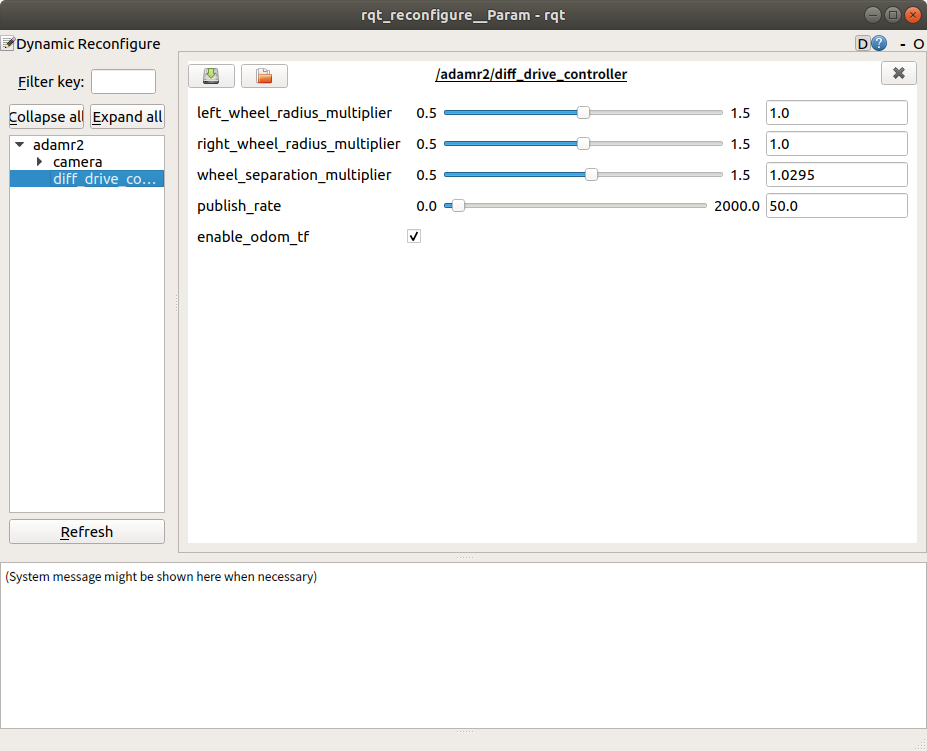
\includegraphics[height=100truemm]{images/dynamic_reconfigure.png}
  \caption{\textsf{dynamic\_reconfigure}}
  \label{fig:dynamic_reconfigure}
\end{figure}

\subsection{移動距離に基づいたオドメトリ調整}

ここでは移動距離に基づいたオーソドックスなオドメトリ調整の手法を紹介します.
オドメトリ調整の手順は単純で,ロボットを一定距離移動させ,実際に移動した距離をメジャー等で測り,オドメトリが示した移動距離と比較するものです.

オドメトリ調整を行う際は,まず直進成分から着手します.
この理由は,オドメトリの回転成分の式には車輪半径と車輪間距離の両方が関係しているのに対し,直進成分の式では車輪半径のみが関係するからです.
2つのパラメータを同時にチューニングするよりも,1つずつ行った方が効率がよく,精度も向上します.

ロボットを起動し,ゲームパッド等で手動操縦して,ロボットを数メートル移動させます.
このとき,ロボットに送る速度指令には旋回成分を含まないようにします.
ロボットの左右の車輪が等しい半径を持つとは限らないからです.
直進指令のみを出したにも関わらずロボットの軌道が曲がったりしたら,左右の車輪半径の係数も調整する必要があります.

オドメトリが計算した移動距離を見るには,\textsf{/adamr2/diff\_drive\_controller/odom}トピックを取得します.
コード\ref{code:echo_adamr2_diff_drive_controller_odom}を実行することで,ターミナルにオドメトリの情報を表示することができます.

\begin{lstlisting}[language=sh, label=code:echo_adamr2_diff_drive_controller_odom, caption=Show Odometry Topic Message]
$ rostopic echo /adamr2/diff_drive_controller/odom
header: 
  seq: 4713
  stamp: 
    secs: 94
    nsecs: 923000000
  frame_id: "odom"
child_frame_id: "base_footprint"
pose: 
  pose: 
    position: 
      x: -1.28079082702
      y: -0.174312002338
      z: 0.0
    orientation: 
      x: -0.0
      y: 0.0
      z: 0.0594169792921
      w: -0.998233250584
  covariance: [0.001, 0.0, 0.0, 0.0, 0.0, 0.0, 0.0, 0.001, 0.0, 0.0, 0.0, 0.0, 0.0, 0.0, 1000000.0, 0.0, 0.0, 0.0, 0.0, 0.0, 0.0, 1000000.0, 0.0, 0.0, 0.0, 0.0, 0.0, 0.0, 1000000.0, 0.0, 0.0, 0.0, 0.0, 0.0, 0.0, 10.0]
twist: 
  twist: 
    linear: 
      x: -0.000235845256857
      y: 0.0
      z: 0.0
    angular: 
      x: 0.0
      y: 0.0
      z: 0.000285137126708
  covariance: [0.001, 0.0, 0.0, 0.0, 0.0, 0.0, 0.0, 0.001, 0.0, 0.0, 0.0, 0.0, 0.0, 0.0, 1000000.0, 0.0, 0.0, 0.0, 0.0, 0.0, 0.0, 1000000.0, 0.0, 0.0, 0.0, 0.0, 0.0, 0.0, 1000000.0, 0.0, 0.0, 0.0, 0.0, 0.0, 0.0, 10.0]
\end{lstlisting}

トピックを受信すると,コード\ref{code:echo_adamr2_diff_drive_controller_odom}のような情報がターミナル上に表示されます.
この内,\textsf{pose}の項の\textsf{position}がロボットの位置,\textsf{orientation}がロボットの回転を表します.
ロボットが直進すると,\textsf{position}の\textsf{x}の値が増加します.
この値を実測値と示し合わせ,実測値よりも小さければ\textsf{wheel\_radius\_multiplier}の値を大きくします.
実測値よりも大きければ,\textsf{wheel\_radius\_multiplier}の値を小さくします.

車輪半径を調整し終えたら,次は車輪トレッドの調整を行います.
車輪トレッドの調整も同様の手順で行えますが,1つ問題なのが\textsf{odom}トピックの回転がクォータニオンで表示されるということです.
クォータニオンをロールピッチヨーに変換するのはさして難しくないのですが,一目見ただけではなかなかわかりません.
従って,測定の際は何らかの工夫をしなければならないということになります.

ここではロボットが2回転するとクォータニオンが元に戻ることを利用して,ロボットを偶数回旋回させた後のオドメトリのデータを見て調整する手法を取ります.
ロボットの起動直後から4回転ほど旋回させ,オドメトリのトピックデータを確認します.
クォータニオンの値がロボットの起動直後と同じ値になっていれば,車輪トレッドの数値は正しいことになります.
もしオドメトリの回転数が実際の回転数(4回分の回転)よりも小さければ,\textsf{wheel\_separation\_multiplier}の値を小さくします.
オドメトリの回転数が実際の回転数よりも大きければ,\textsf{wheel\_separation\_multiplier}の値を大きくします.

この手法でオドメトリ調整を行う際の注意点として,以下の2点があります.

\begin{itemize}
  \item ロボットを移動させるときは\textsf{odom}トピックの値をゼロに近くしてから行うこと.
  \item パラメータの変更はロボットが移動する前に行うこと.
\end{itemize}

\textsf{odom}トピックはロボットのコントローラが起動してからの絶対的な移動距離を示すため,相対的な位置を(直接)求めることができません.
そのため,オドメトリ調整を行う際は\textsf{odom}トピックの位置の値をゼロに近づけてから行う必要があります.
バージョン0.17.1時点での\textsf{diff\_drive\_controller}にはオドメトリの位置をリセットする機能は無いので,
\footnote{GitHubのIssue(\#382)で議論されてはいますが,機能の実装は検討されていないようです.}
ロボットを移動させてから元の位置に戻す他ありません.
オドメトリのパラメータを変更する前ならば,もし車輪半径やトレッドのパラメータが間違っていたとしても,元の動作の反対の動作を行えばオドメトリの原点に復帰することができます.

以上のことに気を付けてオドメトリ調整を行いましょう.

\subsection{レーザースキャナを利用したオドメトリ調整}

オドメトリの調整手段として,レーザースキャナを利用した方法もあります.
こちらは実測値に基づいているわけではないため正確さには欠けますが,レーザースキャナと壁さえあればメジャー等で測定する手間が無いという利点があります.

レーザースキャナを利用したオドメトリ調整の手順を以下に示します.

\begin{enumerate}
  \item ロボットを壁から数メートル離れた箇所に,壁に垂直に向くように設置します.
  \item \textsf{adamr2\_control.launch},\textsf{joy.launch},\textsf{rpidar.launch}を起動して,ロボットが走行可能かつレーザースキャナのデータを閲覧可能な状態にします.
  \item \textsf{rviz}を起動し,\textsf{Fixed Frame}を\textsf{odom}に設定します.
  \item \textsf{rviz}のトピックに\textsf{LaserScan}を追加し,\textsf{LaserScan}トピックのオプションの内,減衰時間(Decay Time)を20秒程度に設定します.
  \item ゲームパッドを使ってロボットを動かします.直進成分の調整を行う場合は壁に向かってまっすぐ走らせ,旋回成分の調整を行う場合はその場でゆっくり旋回させます.
  \item レーザースキャンのデータのズレを確認します.
    \begin{itemize}
      \item オドメトリが正確ならば,20秒間のレーザースキャンは1つのスキャンであるかのように見えるはずです.
      \item オドメトリにズレがあれば,レーザースキャンは重ならず,厚くなったりズレたりします.
    \end{itemize}
  \item \textsf{dynamic\_reconfigure}を使って車輪のパラメータを調整します.
\end{enumerate}

レーザースキャナで壁を測定した結果をもとに,オドメトリのズレを可視化するという手法です.
注意点として,ロボットを旋回させるときは十分にゆっくり旋回させなければなりません.
ロボットに搭載しているレーザースキャナが,レーザーヘッドを回転させて計測するタイプのものであった場合,ロボットが高速で旋回するとスキャンに歪みが生じます.
これを可能な限り減らすために,なるべくゆっくりと旋回させる必要があります.

\end{document}